\subsection{Crossover}
The system performs an uniform crossover. We consider the notes, chords and rests as the alleles that are selected in the offspring. Two parents produce one child and all parents are paired with each other. We get for \(N\) parents \( \frac{N * (N-1)}{2} \) children.

On figure \ref{fig:cross_init} two parents are graphically displayed. During the crossover, we iteratively go over each offset an consider the alleles of both parents on that offset to be selected. Both alleles have an equal chance to be selected. On figure \ref{fig:cross_7} a sample child of the corresponding parents is illustrated.

\begin{figure}[H]
    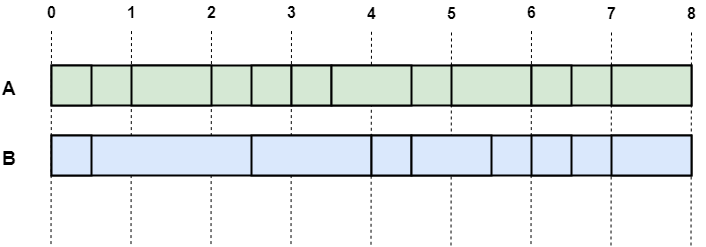
\includegraphics[width=\linewidth]{Fotos/crossover/init.png}
	\caption{Two parents A and B. Each rectangle is considered to be a note, chord or rest with its own size.}
	\label{fig:cross_init}
\end{figure}

\begin{figure}[H]
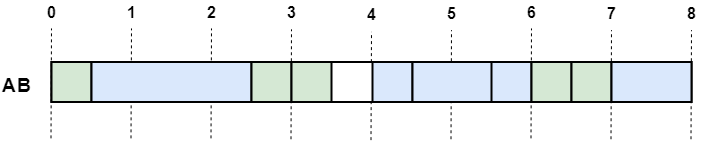
\includegraphics[width=\linewidth]{Fotos/crossover/last.png}
\caption{Offspring of the parents A and B.}
\label{fig:cross_7}
\end{figure}

% TODO fix the array gap.

This process is repeated multiple times during the execution, every song in a group must be paired with every other song. So we get for \(N\) parents \( \frac{N * (N-1)}{2} \) children.


